\documentclass{article}
\usepackage[utf8]{vietnam}
\usepackage{graphicx}
\usepackage{amsmath,amssymb}
\usepackage{tikz}
\usepackage{tikz-3dplot}
\title{BÀI TẬP LỚN NHẬP MÔN ĐIỆN TOÁN}
\author{}
\date{Ngày 29 Tháng 1 Năm 2020}
\begin{document}
\maketitle
\tableofcontents\newpage
\
\section{Autonomous Car là gì?}
Các bạn đã quá quen thuộc với những chiếc xe máy hay ô tô đi trên đường hằng ngày phai không nào? Mỗi phương tiện như vậy đều phải cần có người ngồi lên và điều khiển chúng.Có khi nào bạn ngồi vu vơ nghĩ rằng một ngày nào đó các phương tiện đó không cần người điều khiển chúng nhưng chúng vẫn đến đúng nơi cần đến hay không? Nếu bạn nghĩ đó là vô lí thì mình xin thưa rằng đó không là mơ mà nó đã là hiện thực rồi đó.Vậy xe tự hành là gì ? Xe tự hành là phương tiện có thể tự lái từ điểm xuất phát đến điểm đến định trước ở chế độ “lái tự động” bằng cách sử dụng các công nghệ và cảm biến khác nhau trong xe, bao gồm điều khiển hành trình thích ứng, hệ thống lái chủ động (lái bằng dây), hệ thống chống bó cứng phanh ( phanh bằng dây), công nghệ định vị GPS, laser và radar.Ngoài ra còn có một số ứng dựng thông minh từ các lĩnh vực khoa học máy tính vô cùng hữu ích hứa hẹn là một trong những sản phẩm công nghệ mang tính đột phá trong những năm tới.Ưu điểm vượt trội của xe tự lái là khả năng tự lái an toàn, độ bảo mật tốt, bảo vệ người lái trách những tai nạn không đáng có.

\section{Công nghệ trong Autonomous Car}
\subsection{GPS}
GPS( Global Positioning System), hệ thống GPS giúp xe có thể định vị được chính xác vị trí trên bản đồ. Hệ thống này khá quen thuộc với chúng ta khi mọi thiết bị di động hiện giờ đều tích hợp GPS.Nhờ vào hệ thống định vị GPS,Autonomous Car mới phát huy được bản chất của mình.
\begin{figure}[h]
\centering 
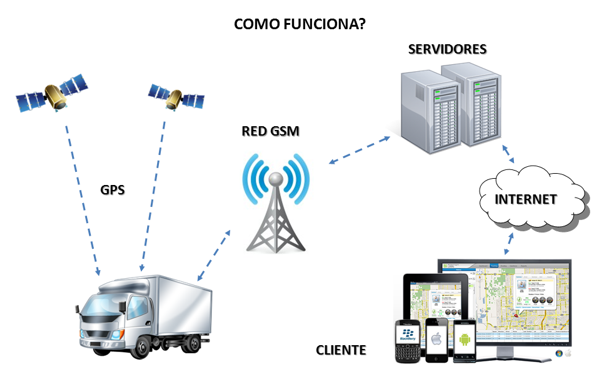
\includegraphics[width=150mm]{1.png} 
\caption{GPS} 
\label{dinhnghia} 
\end{figure}
\subsection{Hệ thống IMU (Inertial Measurement Unit)}
Giúp xe có thể biết được góc quay, gia tốc và vận tốc tuyến tính và góc của xe . Cấu tạo của IMU bao gồm 3 cảm biến cơ bản: cảm biến gia tốc (accelerationmeter), con quay hồi chuyển (gyrosope) và la bàn (compass). Thông thường các giá trị “thô” (raw) của các cảm biến này rất nhiều (noise) vậy nên cần các thuật toán để tổng hợp và xử lý data, đưa ra giá trị tối ưu nhất.
\begin{figure}[h]
\centering 
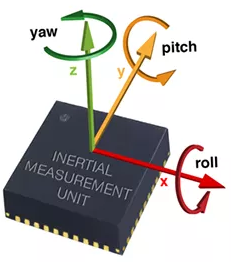
\includegraphics[width=100mm]{3.png} 
\caption{IMU} 
\label{dinhnghia} 
\end{figure}//

\subsection{Cảm biến}
Cảm biến siêu âm ( Ultrasonic sensors) dùng để do khoảng các đối tượng gần xe và được dùng để hỗ trợ đỗ xe.Bộ phận này hỗ trợ xe xử lí tình hướng tốt hơn.
\subsection{Hệ thống }
Hệ thống Lidar (Light detection and ranging) cảm biến này sử dụng chùm tia lazer quay liên tục để đo khoảng cách với tốc độ lấy mẫu cực kỳ cao, số lượng mẫu có thể đạt được 2.2 triệu mẫu /s, và khoảng cách có thể đo được là hơn 120 m. Dữ liệu truyền về sẽ là các mây điểm (point cloud). Việc xử lý các point cloud này đòi hỏi thuật toán rất phức tạp nhằm nhận diện các vật thể xung quanh và xây dựng bản đồ 3D cho xe tự hành. Bạn có thể tham khảo point cloud data của lidar truyền về bên dưới.
\begin{figure}[h]
\centering 
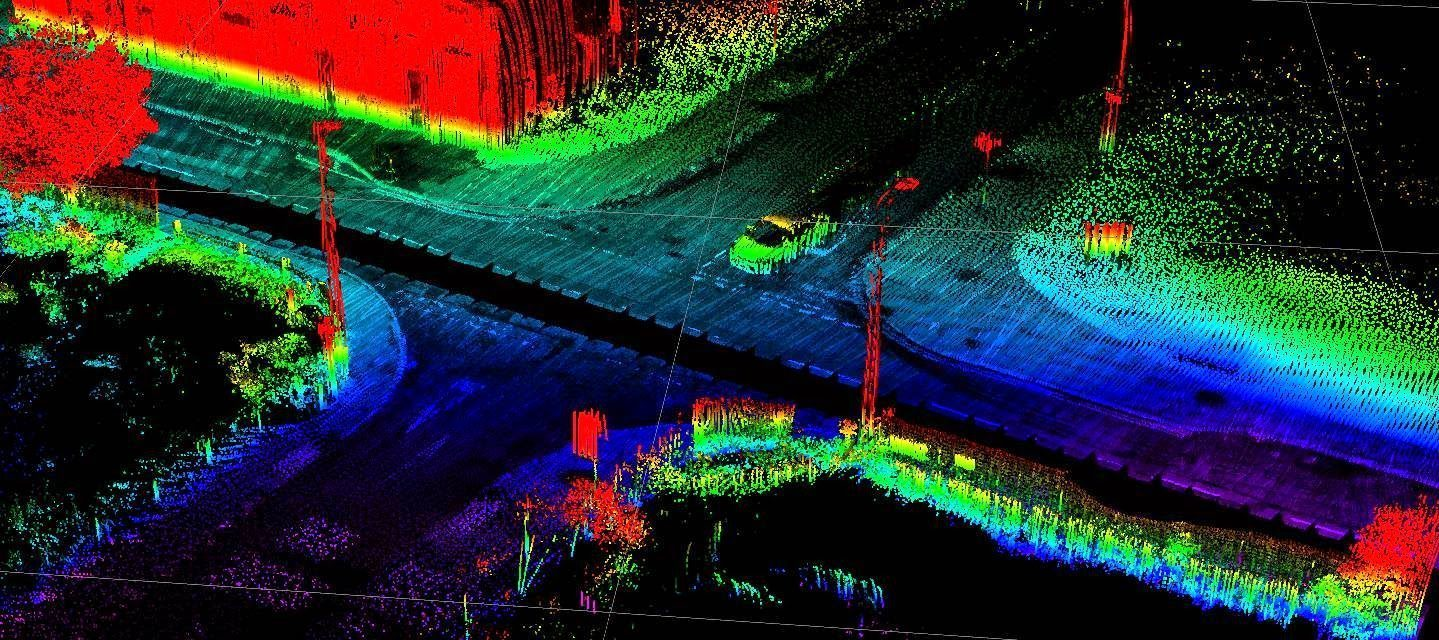
\includegraphics[width=150mm]{5.jpeg} 
\caption{Lindar} 
\label{dinhnghia} 
\end{figure}
\subsection{Camera}
Camera được sử dụng trong xe tự hành thông thường là các dạng camera công nghiệp, được truyền về hệ thống điều khiển thông qua các chuẩn truyền thông công nghiệp như USB3.0, Firewire, Camera Link, Gige,…Hệ thống camera ngày càng được nâng cấp lên 2D thậm chí là 3D, giúp xe quan sát tốt hơn, biết được những vật cản bình thường rất khó thấy bằng mắt thường.
\subsection{Radar}
Hệ thống radar được gắn trước mũi xe, giúp xe có thể phát hiện được các vật cản hoặc các phương tiện phía trước mũi xe, toàn bộ data được truyền về hệ thống điều khiển để giúp xe có thể đưa ra quyết định chính xác để né vật cản
\subsection{Máy tính trung tâm}
Máy tính trung tâm (Center Computer) là hệ thống điều khiển trung tâm dùng để xử lý toàn bộ data cảm biến  đưa về. Các bài toán cần giải quyết ở xe tự hành đó là nhận diện biển báo “sign recognition”, nhận diện làn đường “lane detection”, nhận diện vật cản “obstacle recognition” , … sau khi giải quyết các bài toán trên xe sẽ đưa ra quyết định chính xác đường đi “path finding” của xe, cũng như là dự đoán “prediction” các trường hợp có thể xảy ra trên quá trình di chuyển.
\section{Những thành tựu của Autonomous Car}
Không chỉ đơn giản là những lý thuyết khô khan mà kèm theo đó các nhà khoa học , kĩ sư đã bắt tay và hiện thực các ý tưởng sáng tạo của mình để tạo nên những chiếc xe tự lái mang tính đột phá cao làm tiền đề cho cuộc cách mạng bùng nổ và phát triển. đông thời chúng mang lại những thành tựu vô cùng xuất sắc.
\subsection{Thực hiện hóa ý tưởng về xe tự hành}
Nếu như năm 2016, những chiếc xe tự vận hành không cần người điều khiển mới nằm ở mặt ý tưởng và thử nghiệm sơ khai thì năm 2017, đã ghi nhận những bước tiến gần hơn đến tương lai mà mọi phương tiện tham gia giao thông sẽ không cần con người tham gia điều khiển.

Không chỉ có những tay chơi quen thuộc trong ngành sản xuất ô tô như Honda, Mercedes hay Tesla, giờ đây sân chơi phương tiện tự hành mở ra cho cả những ông lớn công nghệ như Facebook, Google hay Intel.

 

\end{document}
